\documentclass[10pt]{article}

\usepackage{pictex, latexsym, graphicx,amsmath,amssymb,amsbsy,amsfonts,amsthm,verbatim}
\usepackage{graphics}
\usepackage{fullpage}
\usepackage{fancyhdr}

\usepackage{algorithm,algorithmic}
\usepackage{multirow}


\setlength{\voffset}{-0.25in}
\setlength{\headsep}{0.25in}
\setlength{\parskip}{1em}
\setlength{\parindent}{0em}

% Macros
\def\vu{\mathbf{u}}
\def\vx{\mathbf{x}}
\def\vb{\mathbf{b}}
\def\vv{\mathbf{v}}
\def\vw{\mathbf{w}}

\renewcommand{\implies}{\rightarrow}
\renewcommand{\lor}{\vee}
\renewcommand{\land}{\wedge}
\newcommand{\xor}{\oplus}
\renewcommand{\iff}{\leftrightarrow}
\newcommand{\TRUE}{\mathbf{T}}
\newcommand{\FALSE}{\mathbf{F}}
\newcommand{\universe}{\mathcal{U}}

% Counter for the problems.
\newcounter{problem}
\newcommand{\problem}{\textbf{\refstepcounter{problem}Problem \theproblem.} }



% =======================CUSTOM PACKAGES/MACROS===========================
% Numbering with letters
\usepackage{enumitem}
\newcommand{\solution}{\vspace{0.5cm}\textbf{\textit{Solution}} \\}

% Graphs
\usepackage{tkz-graph}
\usepackage{tikz}

\tikzstyle{cn}=[shape=circle,draw] % c = circle; n = normal mode
\tikzstyle{sn}=[shape=rectangle,draw] % s = square/rectangle; n = normal mode
\tikzstyle{from}=[<-,shorten <=1pt,>=stealth,semithick]
\tikzstyle{to}=[->,shorten >=1pt,>=stealth,semithick]
\tikzstyle{common}=[shorten >=1pt,>=stealth,semithick]

% Code
\usepackage{listings}
\usepackage{courier}

\lstset{basicstyle=\footnotesize\ttfamily,breaklines=true}
\lstset{framextopmargin=50pt,frame=bottomline}
% =========================================================================



\begin{document}
\pagestyle{fancyplain}
%%%%%%%%%%%%%%%%%%%%%%%%%%%%%%%%%%
\chead{DISCRETE STRUCTURE (CO1007) - SOLUTION to GRAPH, CONNECTIVITY and TREE}
%\chead{DISCRETE STRUCTURE (CO1007) --- Homework 01 --- PROPOSITIONAL LOGIC}

\begin{center}
    \begin{tabular}{|c|c|c|c|}
        \hline 
        \multicolumn{4}{|c|}{\textbf{GROUP ... ---- MEMBER LIST}} \\ 
        \hline 
        \textbf{No.} &\qquad\qquad \textbf{Name}\qquad\qquad\qquad & \qquad\textbf{ID}\qquad\qquad & \qquad\textbf{Role}\qquad\qquad \\ 
        \hline 
        1 &  &  &  \\ 
        \hline 
        2 &  &  &  \\ 
        \hline 
        3 &  &  &  \\ 
        \hline 
        4 &  &  &  \\ 
        \hline 
        5 &  &  &  \\ 
        \hline 
    \end{tabular} 
\end{center}

\pagebreak

\section{Graph}
% 1
\problem 


\section{Connnectivity}
\setcounter{problem}{0}

% 1
\problem Determine whether each of these graphs is strongly connected and if not, whether it is
weakly connected.

\solution
\begin{enumerate}[label=(\alph*)]
\item The graph is weakly connected. (there is no path from $a$ to other vertices.)
\item The graph is weakly connected. (there is no path from $c$ to other vertices.)
\item The graph is not connected.
\item The graph is not connected.
\item the graph is strongly connected.
\end{enumerate}

% 2
\problem Does each of these lists of vertices form a path in the following graph? Which paths are
simple? Which are circuits? What are the lengths of those that are paths?

\solution
\begin{enumerate}[label=(\alph*)]
\item \textbf{Path(s)}: a, d
\item \textbf{Simple Path(s)}: d
\item \textbf{Circuit(s)}: d
\item \textbf{Length of path(s)}: \\
    \begin{itemize}
        \item a: 4
        \item d: 5
    \end{itemize}
\end{enumerate}

% 3
\problem Does each of these lists of vertices form a path in the following graph? Which paths are
simple? Which are circuits? What are the lengths of those that are paths?

\solution
\begin{enumerate}[label=(\alph*)]
\item \textbf{Path(s)}: a, b
\item \textbf{Simple Path(s)}: a
\item \textbf{Circuit(s)}: no
\item \textbf{Length of path(s)}: \\
    \begin{itemize}
        \item a: 4
        \item d: 4
    \end{itemize}
\end{enumerate}

% 4
\problem Whether the given graph is connected.

\solution
\begin{enumerate}[label=(\alph*)]
\item Not connected
\item Connected
\item Not connected
\end{enumerate}

% 5
\problem How many connected components does each of the graphs in above Exercise have?

\solution
\begin{enumerate}[label=(\alph*)]
\item 3
\item 1
\item 2
\end{enumerate}

% 6
\problem Find the number of paths of length n between two different vertices in $K_{4}$ if
n is a) 2 b) 3

\solution
\begin{enumerate}[label=(\alph*)]
\item Number of paths with length 2: 24
\item Number of paths with length 3: 24
\end{enumerate}

% 7
\problem Find all the cut vertices of the given graphs

\solution
\begin{enumerate}[label=(\alph*)]
\item c
\item c, d
\item b, c, e, i
\end{enumerate}

% 8
\problem Find all the cut vertices of the given graph

\solution
\begin{enumerate}[label=(\alph*)]
\item No
\item cd
\item ab, bc, cd, ce, ei, ih
\end{enumerate}

% 9
\problem Find all the cut vertices, cut edges of the graphs

\solution
\begin{enumerate}[label=(\alph*)]
\item $C_{n}$, where $n \geq 3$: no cut vertices, no cut edges
\item $W_{n}$, where $n \geq 3$: no cut vertices, no cut edges
\item $K_{m, n}$, where $m \geq 2, n \geq 2$: no cut vertices, no cut edges
\end{enumerate}

% 10
\problem For each of these graphs, find $\kappa(G)$; $\lambda(G)$.

\solution
\begin{enumerate}[label=(\alph*)]
\item $\kappa(G) = 1$; $\lambda(G) = 2$
\item $\kappa(G) = 2$; $\lambda(G) = 2$
\end{enumerate}

% 11
\problem Construct a graph $G$ with $\kappa(G) = 1$ $\lambda(G) = 2$ and $min_{v \in V} deg(v) = 3$.

\solution
\vspace{0.5cm}

\begin{center}
    \begin{tikzpicture}        
        \node[cn] (A) at (0, 0) {};
        \node[cn] (B) at (2, 2) {}
            edge[common] node[auto, swap] {} (A)
        ;
        \node[cn] (C) at (2, 0) {}
            edge[common] node[auto, swap] {} (A)
            edge[common] node[auto, swap] {} (B)
        ;
        \node[cn] (D) at (4, 0) {}
            edge[common, bend left] node[auto, swap] {} (A)
            edge[common] node[auto, swap] {} (B)
            edge[common] node[auto, swap] {} (C)
        ;
        \node[cn] (E) at (6, 0) {}
            edge[common, bend left] node[auto, swap] {} (D)
            edge[common, bend right] node[auto, swap] {} (D)
        ;
        \node[cn] (F) at (8, 2) {}
            edge[common] node[auto, swap] {} (E)
        ;
        \node[cn] (G) at (8, 0) {}
            edge[common] node[auto, swap] {} (E)
            edge[common] node[auto, swap] {} (F)
        ;
        \node[cn] (H) at (10, 0) {}
            edge[common, bend left] node[auto, swap] {} (E)
            edge[common] node[auto, swap] {} (F)
            edge[common] node[auto, swap] {} (G)
        ;
    \end{tikzpicture}
\end{center}

% 12
\problem Determine whether the given graph has an Euler circuit. Construct such a circuit when one
exists. If no Euler circuit exists, determine whether the graph has an Euler path and construct such
a path if one exists.

\solution
\begin{enumerate}[label=(\alph*)]
\item No circuit and path
\item Circuit: bdaedghefhifcb
\item Path: acecdbebaed
\item Path: cdecbdabfaef
\item Circuit: eaeabdebcdce
\item Path: bcibaihadefdigdc
\end{enumerate}

% 13
\problem Determine whether the picture shown can be drawn with a pencil in a continuous motion without
lifting the pencil or retracing part of the picture.
\begin{enumerate}[label=(\alph*)]
\item
    \begin{tikzpicture}
        \node[cn] (A) at (0, 0) {};
        \node[cn] (B) at (1.4, 0) {}
            edge[from] node[auto, swap] {2} (A)
        ;
        \node[cn] (C) at (2.8, 0) {}
            edge[from] node[auto, swap] {14} (B)
        ;
        \node[cn] (D) at (4.2, 0) {}
            edge[from] node[auto, swap] {5} (C)
        ;
        \node[cn] (E) at (2.1, -1.4) {}
            edge[from] node[auto, swap] {3} (B)
            edge[to] node[auto, swap] {4} (C)
        ;
        \node[cn] (F) at (0.7, 1.4) {}
            edge[to] node[auto, swap] {1} (A)
            edge[to] node[auto, swap] {13} (B)
        ;
        \node[cn] (G) at (3.5, 1.4) {}
            edge[from] node[auto, swap] {15} (C)
            edge[from] node[auto, swap] {6} (D)
        ;
        \node[cn] (H) at (0, 2.8) {}
            edge[to] node[auto, swap] {12} (F)
        ;
        \node[cn] (I) at (1.4, 2.8) {}
            edge[to] node[auto, swap] {11} (H)
            edge[to] node[auto, swap] {18} (F)
        ;
        \node[cn] (J) at (2.8, 2.8) {}
            edge[to] node[auto, swap] {17} (I)
            edge[from] node[auto, swap] {16} (G)
        ;
        \node[cn] (K) at (4.2, 2.8) {}
            edge[to] node[auto, swap] {8} (J)
            edge[from] node[auto, swap] {7} (G)
        ;
        \node[cn] (L) at (2.1, 4.2) {}
            edge[to] node[auto, swap] {10} (I)
            edge[from] node[auto, swap] {9} (J)
        ;
    \end{tikzpicture}
\item
    \begin{tikzpicture}
        \node[cn] (A) at (0, 4) {}
        ;
        \node[cn] (B) at (-3, 3) {}
        ;
        \node[cn] (C) at (0, 3) {}
            edge[from] node[auto, swap] {1} (A)
            edge[to] node[auto, swap] {2} (B)
        ;
        \node[cn] (D) at (3, 3) {}
            edge[to] node[auto, swap] {7} (C)
        ;
        \node[cn] (E) at (-2, 2) {}
        ;
        \node[cn] (F) at (0, 2) {}
            edge[from] node[auto, swap] {8} (C)
            edge[to] node[auto, swap] {9} (E)
        ;
        \node[cn] (G) at (2, 2) {}
            edge[to] node[auto, swap] {14} (F)
        ;
        \node[cn] (H) at (-1, 1) {}
        ;
        \node[cn] (I) at (0, 1) {}
            edge[from] node[auto, swap] {15} (F)
            edge[to] node[auto, swap] {16} (H)
        ;
        \node[cn] (J) at (1, 1) {}
            edge[to] node[auto, swap] {21} (I)
        ;
        \node[cn] (K) at (-1, -1) {}
            edge[from] node[auto, swap] {17} (H)
        ;
        \node[cn] (L) at (0, -1) {}
            edge[from] node[auto, swap] {22} (I)
            edge[from] node[auto, swap] {18} (K)
        ;
        \node[cn] (M) at (1, -1) {}
            edge[to] node[auto, swap] {20} (J)
            edge[from] node[auto, swap] {19} (L)
        ;
        \node[cn] (N) at (-2, -2) {}
            edge[from] node[auto, swap] {10} (E)
        ;
        \node[cn] (O) at (0, -2) {}
            edge[from] node[auto, swap] {23} (L)
            edge[from] node[auto, swap] {11} (N)
        ;
        \node[cn] (P) at (2, -2) {}
            edge[to] node[auto, swap] {13} (G)
            edge[from] node[auto, swap] {12} (O)
        ;
        \node[cn] (Q) at (-3, -3) {}
            edge[from] node[auto, swap] {3} (B)
        ;
        \node[cn] (R) at (0, -3) {}
            edge[from] node[auto, swap] {24} (O)
            edge[from] node[auto, swap] {4} (Q)
        ;
        \node[cn] (S) at (3, -3) {}
            edge[to] node[auto, swap] {6} (D)
            edge[from] node[auto, swap] {5} (R)
        ;
        \node[cn] (T) at (0, -4) {}
            edge[from] node[auto, swap] {25} (R)
        ;
    \end{tikzpicture}
\end{enumerate}

% 14
\problem For which values of $n$ do these graphs have an Euler circuit?
\begin{enumerate}[label=(\alph*)]
    \item $K_{n}$
    \item $C_{n}$
    \item $W_{n}$
    \item $Q_{n}$
\end{enumerate}

\solution
\par A graph has Euler circuit if and only if each vertex has even degree.
\begin{enumerate}[label=(\alph*)]
    \item $K_{n}$ \\
        \par In a complete graph, each vertex has degree of $n - 1$. \\
        $\Rightarrow (n - 1) \vert \quad 2$ \\
        $\Rightarrow n \not \vert \quad 2$
    \item $C_{n}$
        \par In a cycle, each vertex has degree of 2. Therefore, $n \in \mathbf{N}^{*}$. \\
    \item $W_{n}$
        \par In a wheel, each vertex on the outer cycle has degree of 3. Therefore, $n \in \emptyset$.
    \item $Q_{n}$
        \par In a hypercube, each vertex has degree of $n$. Therefore, $n \vert \quad 2$.
\end{enumerate}

% 15
\problem Determine whether the given graph has a Hamilton circuit. If it does, find such a circuit.
If it does not, give an argument to show why no such circuit exists.

\solution
\par Some properties of Hamilton circuit:
    \begin{itemize}    
        \item A graph with a vertex of degree one cannot have a Hamilton circuit, because in a
            Hamilton circuit, each vertex is incident with two edges in the circuit.
        \item If a vertex in the graph has degree two, then both edges that are incident with this
            vertex must be part of any Hamilton circuit.
        \item When a Hamilton circuit is being constructed and this circuit has passed through a
            vertex, then all remaining edges incident with this vertex, other than the two used in
            the circuit, can be removed from consideration.
        \item A Hamilton circuit cannot contain a smaller circuit within it.
    \end{itemize}    

\begin{enumerate}[label=(\alph*)]
    \item No Hamilton circuit.
        \par Vertices $a$ and $b$ have degree two. Therefore, edges $ab$, $ac$ and $bc$ are would be
        parts of the Hamilton circuit if one exists. Because the two edges $ac$ and $bc$ have been
        parts of the Hamilton circuit, the edge $cf$ cannot be part of the Hamilton circuit.
        Therefore, the is no Hamilton circuit in this graph.
    \item abcdea.
    \item No Hamilton circuit.
        \par This graph has no Hamilton circuit since vertex $f$ has degree one.
    \item No Hamilton circuit.
        \par This graph has no Hamilton circuit since vertex $e$, $f$ and $g$ has degree one.
    \item No Hamilton circuit.
        \par Because vertices $a$, $c$, $g$, $e$ all have degree two, the Hamilton circuit would
        have to contain edges $ab$, $bc$, $ch$, $hg$, $gf$, $fe$, $ed$, $da$. These edges form a
        Hamilton circuit. Because a Hamilton circuit cannot contain a smaller circuit within it,
        this graph does not have a Hamilton circuit.
    \item No Hamilton circuit.
        \par Because vertices $a$, $b$, $c$, $d$ all have degree two, the Hamilton circuit would
        have to contain edges $ab$, $bc$, $cd$, $da$. These edges form a Hamilton circuit. Because a
        Hamilton circuit cannot contain a smaller circuit within it, this graph does not have a
        Hamilton circuit.
\end{enumerate}

% 16
\problem For which values of n do these graphs have an Hamilton circuit?
\begin{enumerate}[label=(\alph*)]
    \item $K_{n}$
    \item $C_{n}$
    \item $W_{n}$
\end{enumerate}

\solution
\begin{itemize}
    \item Any $C_{n}$ has a Hamilton circuit. Since every vertex has degree two, the Hamilton circuit
        would contain all of its edges.
    \item Any $K_{n}$ has a Hamilton circuit. Its circuit would contain all of the edges of its
        subgraph $C_{n}$.
    \item No $W_{n}$ has a Hamilton circuit, because the outer cycle $C_{n}$ forms a Hamilton circuit.
        Meanwhile, Hamilton circuit cannot contain a smaller circuit within it
\end{itemize}

% 17
\problem Find the length of a shortest path between a and z in the given weighted graph.

\solution
%Let a = 0; b = 1; c = 2; d = 3; e = 4; z = 5;
\begin{enumerate}[label=(\alph*)]
    \item 5
%Input:
%6 8 
%0 1 6
%0 2 3
%1 3 5
%1 4 2
%2 4 5
%3 4 1
%3 5 2
%4 5 4
    \item 16
%Input:
%8 12
%0 1 4
%0 2 3
%1 2 2
%1 3 5
%2 3 3
%2 4 6
%3 4 1
%3 5 5
%4 6 5
%5 6 2
%5 7 7
%6 7 4
\end{enumerate}


% 18
\problem Solve the traveling salesperson problem for this graph by finding the total weight of all
Hamilton circuits and determining a circuit with minimum total weight.

\solution
\par The given graph is a $K_{4}$. In a $K_{n}$, there are $(n - 1)! / 2$ different Hamilton circuits.
\par Proof:
\begin{itemize}
    \item A Hamilton circuit is equivalent to an arrangement of vertices. There are $n!$ arrangements.
    \item There are $n$ different vertices. Therefore, there are $n$ different choices of the start
        vertex of each circuit.
    \item For each circuit, there are 2 different directions.
\end{itemize}
\par Therefore, in total, there are $n! / (2n) = (n - 1)! / 2$ different Hamilton circuits
in a $K_{n}$.
\par In the given graph, the are 3 different Hamilton circuit:
\begin{itemize}
    \item abcda: weight $= 3 + 6 + 7 + 2 = 18$.
    \item abdca: weight $= 3 + 4 + 7 + 5 = 19$.
    \item adbca: weight $= 2 + 4 + 6 + 5 = 17$. (minimum weight)
\end{itemize}


% 19
\problem Use Floyd-Warshall to find shortest path between two vertices in a weighted graph.

\solution
\textbf{Implementation in C++} \\
\textbf{Description}
\begin{itemize}
    \item Input: \\
    The first line includes the number of vertices $n_{v}$ and the number of edges $n_{e}$. \\
    For the next $n_{e}$ lines, each line describes 1 edge: start vertex, end vertex and weight of
        that edge. Note that the label of each vertex are mapped from characters to numbers (A = 0, B = 1, etc.)
    \item Output: \\
        Distance matrix generated by using the Floyd-Warshall algorithm. (The output is then
        formatted into a table for better observation).
\end{itemize}

\textbf{Code} \\

\begin{lstlisting}[language=C++]
#include <algorithm> // std::fill
#include <iostream>
#include <utility> // std::pair
#include <vector>


using namespace std;


const int INF = (int) 1e6;
vector<vector<int>> dist;


int main() {

    /*** Get number of vertices and edges ***/
    int nVertices, nEdges;
    cin >> nVertices >> nEdges;

    /*** Generate distance matrix ***/
    dist.resize(nVertices);
    for (int i = 0; i < nVertices; i++) {
        dist[i].resize(nVertices);
        fill(dist[i].begin(), dist[i].end(), INF);
    }

    for (int i = 0; i < nVertices; i++) {
        dist[i][i] = 0;
    }

    /*** Get edges and generate fill distance matrix ***/
    for (int i = 0; i < nEdges; i++) {
        int u, v, w;
        cin >> u >> v >> w;
        dist[u][v] = w;
    }

    /*** Floyd-Warshall ***/
    for (int k = 0; k < nVertices; k++) {
        for (int i = 0; i < nVertices; i++) {
            for (int j = 0; j < nVertices; j++) {
                dist[i][j] = min(dist[i][j], dist[i][k] + dist[k][j]);
            }
        }
    }

    /*** Output ***/
    for (int i = 0; i < nVertices; i++) {
        for (int j = 0; j < nVertices; j++) {
            if (dist[i][j] == INF) {
                cout << "inf ";
            }
            else {
                cout << dist[i][j] << " ";
            }
        }
        cout << "\n";
    }
    return(0);
}
\end{lstlisting}

\textbf{Input} \\
8 17 \\
0 1 8 \\
0 3 6 \\
0 6 7 \\
1 0 3 \\
1 2 2 \\
1 3 1 \\
2 4 2 \\
2 5 5 \\
3 4 4 \\
3 6 1 \\
4 5 9 \\
4 7 1 \\
5 2 4 \\
5 7 3 \\
6 0 5 \\
6 7 4 \\
7 5 7 \\

\textbf{Output} \\
0 8 10 6 10 15 7 11 \\
3 0 2 1 4 7 2 5 \\
inf inf 0 inf 2 5 inf 3 \\
6 14 16 0 4 12 1 5 \\
inf inf 12 inf 0 8 inf 1 \\
inf inf 4 inf 6 0 inf 3 \\
5 13 15 11 15 11 0 4 \\
inf inf 11 inf 13 7 inf 0 \\

\begin{tabular}{|c|c|c|c|c|c|c|c|c|}
      & A        & B        & C  & D        & E  & F  & G        & H \\
    \hline
    A & 0        & 8        & 10 & 6        & 10 & 15 & 7        & 11 \\
    \hline
    B & 3        & 0        & 2  & 1        & 4  & 7  & 2        & 5 \\
    \hline
    C & $\infty$ & $\infty$ & 0  & $\infty$ & 2  & 5  & $\infty$ & 3 \\
    \hline
    D & 6        & 14       & 16 & 0        & 4  & 12 & 1        & 5 \\
    \hline
    E & $\infty$ & $\infty$ & 12 & $\infty$ & 0  & 8  & $\infty$ & 1 \\
    \hline
    F & $\infty$ & $\infty$ & 4  & $\infty$ & 6  & 0  & $\infty$ & 3 \\
    \hline
    G & 5        & 13       & 15 & 11       & 15 & 11 & 0        & 4 \\
    \hline
    H & $\infty$ & $\infty$ & 11 & $\infty$ & 13 & 7  & $\infty$ & 0 \\
    \hline
\end{tabular}

% 20
\problem Draw the given planar graph without any crossings.

\solution
\begin{enumerate}[label=(\alph*)]
    \item
    \begin{tikzpicture}
        \node[cn] (A) at (0, 2) {}
        ;
        \node[cn] (B) at (0, 4) {}
            edge[common] node[auto, swap] {} (A)
        ;
        \node[cn] (C) at (2, 4) {}
            edge[common] node[auto, swap] {} (B)
        ;
        \node[cn] (D) at (2, 2) {}
            edge[common] node[auto, swap] {} (C)
            edge[common] node[auto, swap] {} (A)
        ;
        \node[cn] (E) at (4, 0) {}
            edge[common] node[auto, swap] {} (C)
            edge[common] node[auto, swap] {} (A)
        ;
    \end{tikzpicture}
    \item
    \begin{tikzpicture}
        \node[cn] (A) at (0, 0) {}
        ;
        \node[cn] (B) at (2, 0) {}
            edge[common] node[auto, swap] {} (A)
        ;
        \node[cn] (C) at (4, 0) {}
            edge[common] node[auto, swap] {} (B)
        ;
        \node[cn] (D) at (2, 2) {}
            edge[common] node[auto, swap] {} (A)
            edge[common] node[auto, swap] {} (C)
        ;
        \node[cn] (E) at (2, 4) {}
            edge[common] node[auto, swap] {} (A)
            edge[common] node[auto, swap] {} (C)
        ;
    \end{tikzpicture}
    \item
    \begin{tikzpicture}
        \node[cn] (A) at (3, 2) {};
        \node[cn] (B) at (0, 0) {}
            edge[common] node[auto, swap] {} (A)
        ;
        \node[cn] (C) at (2, 0) {}
            edge[common] node[auto, swap] {} (A)
            edge[common] node[auto, swap] {} (B)
        ;
        \node[cn] (D) at (4, 0) {}
            edge[common] node[auto, swap] {} (A)
            edge[common, bend left] node[auto, swap] {} (B)
            edge[common] node[auto, swap] {} (C)
        ;
        \node[cn] (E) at (6, 0) {}
            edge[common] node[auto, swap] {} (A)
            edge[common, bend left] node[auto, swap] {} (B)
            edge[common] node[auto, swap] {} (D)
        ;
    \end{tikzpicture}
\end{enumerate}


% 21
\problem Determine whether the given graph is planar. If so, draw it so that no edges cross.

\solution
\begin{enumerate}[label=(\alph*)]
    \item No planar graph
    \item 
        \begin{tikzpicture}
            \node[cn] (A) at (2, 2) {A}
            ;
            \node[cn] (F) at (4, 2) {F}
                edge[common] node[auto, swap] {} (A)
            ;
            \node[cn] (D) at (0, 0) {D}
                edge[common] node[auto, swap] {} (A)
            ;
            \node[cn] (B) at (2, 0) {B}
                edge[common] node[auto, swap] {} (D)
            ;
            \node[cn] (E) at (4, 0) {E}
                edge[common] node[auto, swap] {} (B)
            ;
            \node[cn] (C) at (6, 0) {C}
                edge[common] node[auto, swap] {} (F)
                edge[common] node[auto, swap] {} (E)
                edge[common, bend left] node[auto, swap] {} (D)
            ;
        \end{tikzpicture}
\end{enumerate}


% 22
\problem Construct the dual graph for the map shown. Then find the number of colors needed to color
the map so that no two adjacent regions have the same color.

\solution
\begin{enumerate}[label=(\alph*)]
    \item
        \par Number of colors needed: 4
        \begin{tikzpicture}
            \node[cn] (A) at (3, 2) {A};
            \node[cn] (B) at (0, 0) {B}
                edge[common] node[auto, swap] {} (A)
            ;
            \node[cn] (C) at (2, 0) {C}
                edge[common] node[auto, swap] {} (A)
                edge[common] node[auto, swap] {} (B)
            ;
            \node[cn] (D) at (4, 0) {D}
                edge[common] node[auto, swap] {} (A)
                edge[common, bend left] node[auto, swap] {} (B)
                edge[common] node[auto, swap] {} (C)
            ;
            \node[cn] (E) at (6, 0) {E}
                edge[common] node[auto, swap] {} (A)
                edge[common, bend left] node[auto, swap] {} (B)
                edge[common] node[auto, swap] {} (D)
            ;
        \end{tikzpicture}
    \item
        \par Number of colors needed: 2
        \begin{tikzpicture}
            \node[cn] (A) at (0, 0) {A}
            ;
            \node[cn] (B) at (2, 0) {B}
                edge[common] node[auto, swap] {} (A)
            ;
            \node[cn] (C) at (4, 0) {C}
                edge[common] node[auto, swap] {} (B)
            ;
            \node[cn] (D) at (6, 0) {D}
                edge[common] node[auto, swap] {} (C)
            ;
        \end{tikzpicture}
\end{enumerate}

% 23
\problem What is the chromatic number of $W_{n}$?

\solution
\par The outer cycle has $n - 1$ vertices.
\par If $n - 1 \vert \quad 2$, there needs to be 2 different colors to color the outer cycle.
Therefore, the total number of different colors is 3.
\par If $n - 1 \not \vert \quad 2$, there needs to be 3 different colors to color the outer cycle.
Therefore, the total number of different colors is 4.

\section{Tree}

\textbf{\textit Problem 20}
Find a spanning tree for each of these graphs.
\begin{enumerate}[label=(\alph*)]
    \item $K_{5}$
    \item $K_{4, 4}$
    \item $W_{5}$
    \item $K_{5}$
\end{enumerate}

\solution
\begin{enumerate}[label=(\alph*)]
    \item $K_{5}$
        \begin{tikzpicture}
            \node[cn] (A) at (1.3, 0) {}
            ;
            \node[cn] (B) at (0, -0.95) {}
                edge[common] node[auto, swap] {} (A)
            ;
            \node[cn] (C) at (2.61, -0.95) {}
                edge[common] node[auto, swap] {} (A)
            ;
            \node[cn] (D) at (0.5, -2.48) {}
                edge[common] node[auto, swap] {} (A)
            ;
            \node[cn] (E) at (2.1, -2.48) {}
                edge[common] node[auto, swap] {} (A)
            ;
        \end{tikzpicture}
    \item $K_{4, 4}$
        \begin{tikzpicture}
            \node[cn] (A) at (0, 0) {}
            ;
            \node[cn] (B) at (0, 1) {}
                edge[common] node[auto, swap] {} (A)
            ;
            \node[cn] (C) at (1, 0) {}
                edge[common] node[auto, swap] {} (B)
            ;
            \node[cn] (D) at (1, 1) {}
                edge[common] node[auto, swap] {} (C)
            ;
            \node[cn] (E) at (2, 0) {}
                edge[common] node[auto, swap] {} (D)
            ;
            \node[cn] (F) at (2, 1) {}
                edge[common] node[auto, swap] {} (E)
            ;
            \node[cn] (G) at (3, 0) {}
                edge[common] node[auto, swap] {} (F)
            ;
            \node[cn] (H) at (3, 1) {}
                edge[common] node[auto, swap] {} (G)
            ;
        \end{tikzpicture}
    \item $W_{5}$
        \begin{tikzpicture}
            \node[cn] (A) at (1.3, 0) {}
            ;
            \node[cn] (B) at (0, -0.95) {}
                edge[common] node[auto, swap] {} (A)
            ;
            \node[cn] (C) at (2.61, -0.95) {}
                edge[common] node[auto, swap] {} (A)
            ;
            \node[cn] (D) at (0.5, -2.48) {}
                edge[common] node[auto, swap] {} (B)
            ;
            \node[cn] (E) at (2.1, -2.48) {}
                edge[common] node[auto, swap] {} (C)
            ;
            \node[cn] (F) at (1.3, -1.5) {}
                edge[common] node[auto, swap] {} (A)
            ;
        \end{tikzpicture}
    \item $K_{1, 6}$
        \begin{tikzpicture}
            \node[cn] (A) at (0, 0) {}
            ;
            \node[cn] (B) at (1, 0) {}
            ;
            \node[cn] (C) at (2, 0) {}
            ;
            \node[cn] (D) at (3, 0) {}
            ;
            \node[cn] (E) at (4, 0) {}
            ;
            \node[cn] (F) at (5, 0) {}
            ;
            \node[cn] (G) at (2.5, 2) {}
                edge[common] node[auto, swap] {} (A)
                edge[common] node[auto, swap] {} (B)
                edge[common] node[auto, swap] {} (C)
                edge[common] node[auto, swap] {} (D)
                edge[common] node[auto, swap] {} (E)
                edge[common] node[auto, swap] {} (F)
            ;
        \end{tikzpicture}
\end{enumerate}



\textbf{\textit Problem 21}
Use depth-first search, breath-first search to produce a spanning tree for the given simple graph.
Choose a as the root of this spanning tree and assume that the vertices are ordered alphabetically.

%Input:
%10 12
%0 1
%0 2
%1 2
%2 3
%3 4
%3 5
%4 5
%4 6
%5 7
%6 7
%6 8
%7 8

\solution
\begin{itemize}
    \item Breadth-first Search: a - b - c - d - e - f - g - h - i - j
    \item Depth-first Search: a - b - c - d - e - f - g - i - h - j
\end{itemize}



\textbf{\textit Problem 22}
Use Prim’s algorithm, Kruskal’s algorithm to find a minimum spanning tree for the given weighted
graph.

\solution
\begin{enumerate}[label=(\alph*)]
% IN
%9 16
%0 1 5
%0 3 2
%1 2 4
%1 3 3
%1 4 5
%1 5 6
%2 5 3
%3 4 7
%3 6 6
%3 7 8
%4 5 1
%4 7 3
%5 7 4
%5 8 4
%6 7 4
%7 8 2
    \item Prim's algorithm: \\
% OUT
%Min Cost: 22
%3 - 2
%1 - 3
%2 - 4
%5 - 3
%4 - 1
%7 - 3
%8 - 2
%6 - 4
    Begin the minimum spanning tree at vertex $a$. The tree expands in the following order: \\
    $ad - db - bc - cf - fe - eh - hi - hg$ \\
    Total cost: 22

    \item Kruskal's algorithm: \\
% OUT
%Min cost: 22
%u = 4 v = 5 w = 1
%u = 0 v = 3 w = 2
%u = 7 v = 8 w = 2
%u = 1 v = 3 w = 3
%u = 2 v = 5 w = 3
%u = 4 v = 7 w = 3
%u = 1 v = 2 w = 4
%u = 6 v = 7 w = 4
    The edges are added to the minimum spanning tree in the following order: \\
    $ef(1) - ad(2) - hi(2) - bd(3) - cf(3) - eh(3) - bc(4) - gh(4)$ \\
    Total cost: 22

\end{enumerate}

\end{document}

